
\chapter{Υποσύστημα κίνησης}
\label{ch:motor}

Στο κεφάλαιο Κατασκευή (σ.~\pageref{ch:construction}) αναλύθηκαν τα συστατικά
στοιχεία και οι επιμέρους διατάξεις που συνθέτουν τη φυσική υπόσταση της
συσκευής, μέρος του οποίου είναι αφιερωμένο στους
άξονες κίνησης. Όπως αναφέρεται σε εκείνο το κεφάλαιο, οι μετρήσεις
πραγματοποιούνται από ένα κινητό εξάρτημα της συσκευής, την κεφαλή, που
μετακινείται στο χώρο που ορίζουν αυτοί οι τρεις, στον αριθμό, άξονες.

\begin{figure}
    \caption{Υποσύστημα κίνησης.\label{fig:motor:lvl-0}}
    \begin{center}
    \includegraphics{drive_lvl-0}
    \end{center}
\end{figure}

Στο παρόν κεφάλαιο αναλύεται η διασύνδεση του μικροελεγκτή με τους κινητήρες και
συμπληρωματικές ηλεκτρονικές και μηχανικές διατάξεις για την ανάπτυξη ενός
συστήματος ελέγχου της μετατόπισης της κεφαλής (βλ. σχήμα
\ref{fig:motor:lvl-0}).

Τρεις σερβοκινητήρες συνεχούς περιστροφικής κίνησης (εφεξής, κινητήρες) -- ένας
για κάθε άξονα -- χρησιμοποιούνται για την παραγωγή κίνησης με γωνιακή ταχύτητα
που ελέγχεται μέσω ενός σήματος από παλμούς κυμαινόμενου πλάτους, την
αναφερόμενη ως διαμόρφωση PWM (\te{Pulse-Width Modulation}).
% Something more on PWM (such as averaging voltage).
Αρχικά, αναλύονται
τα διαθέσιμα κυκλώματα Χρονομετρητών\slash{}Απαριθμητών (\te{Timer\slash{}%
Counter}) του μικροελεγκτή που υποστηρίζουν παραγωγή σήματος PWM και
συγκρίνονται τα χαρακτηριστικά τους σε σχέση με τις απαιτήσεις των κινητήρων και
της υλοποίησης προκειμένου να επιλεγεί και διευθετηθεί το πλέον κατάλληλο
(\nameref{sec:motor:motion} σ.~\pageref{sec:motor:motion}).

% (Διευθέτηση γεννήτριας PWM)
% Κάτι σχετικό με κύκλο εργασίας; ???
% PWM για την παραγωγή μίας μέσης τάσης που μετατρέπεται (από τον κινητήρα)

Εν συνεχεία, στην ενότητα Δρομολόγηση (σ.~\pageref{sec:motor:routing})
αναφέρεται η βασική ανάγκη για πολύπλεξη ορισμένων γραμμών ελέγχου, όπως οι
γραμμές σήματος PWM, ώστε να είναι δυνατό να υποστηριχθούν και οι τρεις
κινητήρες μέσω του περιορισμένου αριθμού ακροδεκτών που δύνανται να παράγουν
σήμα PWM.
Στην ενότητα Διεκπεραίωση (σ.~\pageref{subsec:motor:autoshut}) περιγράφεται η
ανάπτυξη ενός μηχανισμού που επιτρέπει το ίδιο το υλικό του μικροελεγκτή να
σταματά την κίνηση των κινητήρων όταν ολοκληρώνεται μία προκαθορισμένη
μετατόπιση, ώστε να εξασφαλίζεται ότι η κεφαλή ακινητοποιείται ακόμα και εάν τη
στιγμή εκείνη, η CPU του μικροελεγκτή είναι απασχολημένη με άλλες εργασίες.
Στην ίδια ενότητα παρουσιάζεται πώς, τελικά, επιτυγχάνεται ταυτόχρονη κίνηση της
κεφαλής στο επίπεδο X-Y (\nameref{ssubsec:motor:common-translation} σ.~%
\pageref{ssubsec:motor:common-translation}).

\begin{figure}
    \caption{\label{fig:motor:lvl-1}}
    \begin{center}
    \includegraphics{drive_lvl-1}
    \end{center}
\end{figure}

Το κεφάλαιο ολοκληρώνεται με την περιγραφή ορισμένων συμπληρωματικών
μηχανισμών, του Εγκλωβισμού και επανάκαμψης (σ.~\pageref{sec:motor:backtrack})
και της Παλιννόστησης (σ.~\pageref{subsec:motor:homing}). Ο μηχανισμός του
εγκλωβισμού προφυλάσσει τη συσκευή
από την πρόκληση βλαβών, κυρίως στους κινητήρες, επιβάλλοντας την ακινητοποίησή
της όταν
η κεφαλή προσκρούει στα άκρα της συσκευής. Λόγω της κρισιμότητας της λειτουργίας
του, ο εγκλωβισμός υλοποιείται σε μηχανικό επίπεδο με χρήση ανασταλτικών
διακοπτών. Οι διακόπτες χρησιμοποιούνται ως έναυσμα για το λογισμικό το οποίο,
με τη σειρά του, προκαλεί την επαναφορά της κεφαλής σε μία γνωστή θέση (τη θέση
επιστροφής) (βλ. Παλιννόστηση σ.~\pageref{subsec:motor:homing}).
Επιπλέον περιγράφεται πώς η συσκευή αποπειράται εκ νέου, και για μία μόνο ακόμη
φορά, τη μετακίνηση στη θέση που είχε προηγουμένως προκαλέσει εγκλωβισμό. Αυτό
συμβαίνει ώστε να εξαλείφεται το ενδεχόμενο ότι ο εγκλωβισμός οφειλόταν σε
αδυναμία παρακολούθησης της πραγματικής θέσης της κεφαλής (αστοχία υλικού) και
που ίσως πλέον καταστεί δυνατό λόγω της πρόσφατης επαναφοράς της κεφαλής στη
θέση επιστροφής (λειτουργία επανάκαμψης).

Η λογική συσχέτιση μεταξύ των μονάδων του υποσυστήματος κίνησης περιγράφεται από
το σχήμα \ref{fig:motor:lvl-1} ενώ η ανάλυσή τους πραγματοποιείται στις επόμενες
ενότητες.

%
% Κινητήρες
%
%\section{Κινητήρες}

\section{Συντεταγμένες και Λειτουργικό εύρος}
\label{sec:motor:coordinates}

Τρεις άξονες γραμμικής κίνησης χρησιμοποιούνται για τη μετακίνηση της κεφαλής
πάνω από την επιφάνεια του παρακολουθούμενου υλικού και κατακορύφως προς και από
αυτό για την πραγματοποίηση μετρήσεων.
Οι άξονες υποδιαιρούνται σε ένα πλήθος νοητών διακριτών θέσεων στις οποίες
μπορεί να μεταβεί η κεφαλή. Το πλήθος αυτών των θέσεων εξαρτάται από την
ελάχιστη δυνατή μετατόπιση που μπορεί να διανύσει η κεφαλή καθώς και το συνολικά
διαθέσιμο μήκος των αντίστοιχων ραγών της συσκευής (πάνω στις οποίες κινείται η
κεφαλή). Στο πλαίσιο της υλοποίησης, η ελάχιστη μετατόπιση ορίζεται ως μία
πλήρης περιστροφή του κινητήρα του αντίστοιχου άξονα. Πρακτικά, αυτό συνεπάγεται
μετατοπίσεις των 4cm, περίπου. Επιπλέον, επιλέγεται να υποστηρίζεται ένα μέγιστο
πλήθος 255 μετατοπίσεων ανά άξονα, δηλαδή ένα μέγιστο μήκος 1km ανά ράγα.

Σε κάθε περίπτωση, το διαθέσιμο πλήθος θέσεων της κεφαλής ορίζουν το αναφερόμενο
ως λειτουργικό εύρος του οποίου η μέγιστη τιμή εξαρτάται άμεσα από τις
διαστάσεις των ραγών της συσκευής. Ωστόσο, προκειμένου να παρέχεται
μεγαλύτερη ευελιξία, το υποσύστημα κίνησης είναι δυνατό να διευθετείται δυναμικά
μέσω λογισμικού ώστε να λειτουργεί σε ένα προσαρμοσμένο λειτουργικό εύρος,
υποσύνολο του μέγιστου δυνατού (βλ. \nameref{subsec:network:config} σ.~%
\pageref{subsec:network:config}).
Η δυνατότητα αυτή επιτρέπει την παρακολούθηση μικρότερων επιφανειών από τη
μέγιστη υποστηριζόμενη. Το σχήμα

\begin{figure}
    \caption{Συντεταγμένες και Λειτουργικό εύρος.\label{fig:motor:coordinates}}
    Σημειώνεται ότι οι συνιστώσες των  συντεταγμένων αριθμούνται από το 0, ενώ
    το λειτουργικό εύρος (το οποίο αντιπροσωπεύει μέγεθος διάστασης) από το 1.
    \begin{center}
    \includegraphics{drive_coordinates}
    \end{center}
\end{figure}


Την κάθε στιγμή, η θέση της κεφαλή προσδιορίζεται από τρεις τιμές· μία για τη
θέση που κατέχει στον άξονα X, μία για τον άξονα Y και μία για το Z, που
συνολικά αναφέρονται ως οι συντεταγμένες (της θέσης) της κεφαλής. Προφανώς,
η κεφαλή μπορεί να τεθεί μόνο σε συντεταγμένες που βρίσκονται εντός του
τρέχοντος λειτουργικού εύρους (είτε αυτό είναι το μέγιστο δυνατό είτε
προσαρμοσμένο).


\section{Παραγωγή κίνησης}
\label{sec:motor:motion}

Σύμφωνα με εγχειρίδιο χρήσης της \textcite{hitec02}, όλοι οι κινητήρες της
λειτουργούν σε τάση 4.8--6V δεχόμενοι τετραγωνικό σήμα ελέγχου με διαμόρφωση
PWM (\textenglish{Pulse-Width Modulation}) 3--5V σε συχνότητα ανανέωσης 50Hz.
Η διάρκεια των παλμών κυμαίνεται μεταξύ 0.9ms και 2.1ms, με παλμούς των 1.5ms να
χρησιμοποιούνται για την ακινητοποίησή τους \parencite{hitec02}.

Οι παραγωγή των παλμών μπορεί να πραγματοποιηθεί είτε με λογισμικό είτε από
κάποιο διαθέσιμο κύκλωμα Χρονομετρητή\slash Απαριθμητή (\textenglish{Timer\slash
Counter}) του μικροελεγκτή. Το κύριο πλεονέκτημα του λογισμικού είναι η
ελευθερία επιλογής οποιουδήποτε ακροδέκτη για την έξοδο του σήματος καθώς και η
δυνατότητα παραγωγής πολλαπλών τέτοιων σημάτων που περιορίζονται από το συνολικό
πλήθος ακροδεκτών ή τη συχνότητα του ρολογιού συστήματος (όποιο είναι
μικρότερο).

Αντιθέτως, στην περίπτωση χρήσης κυκλωμάτων, το παραγόμενο σήμα διοχετεύεται
στους συγκεκριμένους ακροδέκτες με τους οποίους είναι το καθένα εσωτερικά
συνδεδεμένο και, σαφώς, το μέγιστο πλήθος παράλληλων σημάτων περιορίζεται από το
συνολικό αριθμό τέτοιων κυκλωμάτων. Επίσης, κάθε Χρονομετρητής\slash Απαριθμητής
υπόκειται σε πρόσθετους περιορισμούς, όπως το εύρος τιμών που υποστηρίζει ο
καθένας (για παράδειγμα, ανάλυση 8- ή 16-bit).

Ωστόσο, στη χρήση κυκλώματος Χρονομετρητή\slash Απαριθμητή συγκαταλέγονται και
ορισμένα σημαντικά πλεονεκτήματα.
Καθότι το σήμα παράγεται από ξεχωριστό κύκλωμα, η CPU του μικροελεγκτή είναι
διαθέσιμη για την εκτέλεση οποιασδήποτε άλλης εργασίας (για παράδειγμα, κάποιας
ρουτίνας εξυπηρέτησης διακοπής) παράλληλα με την παραγωγή του σήματος, χωρίς να
απαιτείται πολύπλεξη εργασιών (ώστε να αποδίδονται κβάντα τόσο στη γεννήτρια
σήματος όσο και σε κάποια άλλη εργασία). Ένα δεύτερο, λιγότερο σημαντικό για την
προκειμένη υλοποίηση, πλεονέκτημα είναι η δυνατότητα επίτευξης υψηλότερων
συχνοτήτων με πολύ λιγότερο θόρυβο (\textenglish{jitter}) και μεγαλύτερη
ακρίβεια.

Τελικά, για την παραγωγή σήματος PWM των κινητήρων επιλέγεται η χρήση κυκλώματος
Χρονομετρητή\slash Απαριθμητή καθώς, επιπροσθέτως των ανωτέρω πλεονεκτημάτων,
παρουσιάζει υψηλότερο ενδιαφέρον, από εκπαιδευτικής πλευράς.


\subsection{Γεννήτρια PWM}

Ο μικροελεγκτής ATmega328P διαθέτει δύο κυκλώματα Χρονομετρητή\slash Απαριθμητή
με δυνατότητα παραγωγής σήματος PWM. Ο πρώτος (Timer\slash Counter0) είναι 8-bit
και ο δεύτερος (Timer\slash Counter1), 16-bit. Για την επιλογή κάποιου, κρίνεται
σκόπιμη η περαιτέρω ανάλυση της λειτουργίας της γεννήτριας PWM καθώς και των
απαιτήσεων για το σήμα ελέγχου των κινητήρων.

Όσον αφορά τη γεννήτρια PWM, ο Χρονομετρητής\slash Απαριθμητής διαθέτει έναν
καταχωρητή μετρητή, τον TCNTn, ο οποίος σταδιακά αυξάνεται. Επίσης, διαθέτει
δύο ακόμα καταχωρητές, τους OCRnA και OCRnB, οι οποίοι αντιστοιχίζονται με
ακροδέκτες του μικροελεγκτή, αναφερόμενοι ως OCnA και OCnB. Μόλις η τιμή του
TCNTn γίνει ίση με την τιμή που περιέχεται είτε στον OCRnA είτε στον OCRnB,
είναι δυνατή η αλλαγή της εξόδου του αντίστοιχου ακροδέκτη. Ο TCNTn συνεχίζει
την ανοδική του πορεία έως ότου φτάσει την τιμή TOP. Από το σημείο αυτό και
ανάλογα με τη λειτουργία που έχει επιλεγεί, ο TCNTn είτε επανέρχεται ακαριαία
στην τιμή 0 και αρχίζει εκ νέου τον επόμενο κύκλο, είτε φθίνει σταδιακά μέχρι το
0, πάντα εναλλάσσοντας την τιμή των OCnA και OCnB όποτε εξισώνεται με τους OCRnA
και OCRnB, αντιστοίχως \parencite[100--102,124--129]{atmel13}.
Γίνεται αντιληπτό ότι η συχνότητα με την οποία αυξάνεται ο TCNTn καθώς και η
τιμή TOP επηρεάζουν τη συχνότητα του παραγόμενου σήματος. Παράλληλα, η τιμή των
OCRnA και OCRnB επηρεάζουν τον κύκλο εργασίας του (\textenglish{duty cycle}),
δηλαδή το τμήμα της περιόδου κατά το οποίο το παραγόμενο σήμα βρίσκεται σε
λογικό 1.

Η παραγωγή PWM υποστηρίζεται από τρεις ρυθμίσεις λειτουργίας των
Χρονομετρητών\slash Απαριθμητών, τις \textenglish{Fast PWM mode, Phase Correct
PWM mode (PCPWM)} και \textenglish{Phase and Frequency Correct PWM mode
(PFCPWM)}, εκ των οποίων οι δύο τελευταίες ενδείκνυνται για τον έλεγχο κινητήρων
εν γένει, και αυτό επειδή το παραγόμενο σήμα ανταποκρίνεται πιο ομαλά στις
αλλαγές της τιμής TOP \parencite[126,128]{atmel13}. Οι PCPWM και PFCPWM, εφόσον
η τιμή TOP -- η τιμή μέχρι την οποία αυξάνει ο TCNTn πριν αρχίσει τη φθίνουσα
πορεία του -- διατηρείται σταθερή κατά τη διάρκεια λειτουργίας του μετρητή,
είναι πανομοιότυπες \parencite[127]{atmel13}. Στην περίπτωση της υλοποίησης, η
συχνότητα του παραγόμενου σήματος είναι σταθερή, όπως έχει αναφερθεί, στα 50Hz
και, συνεπώς, το ίδιο ισχύει για την τιμή TOP. Ως αποτέλεσμα, οι λειτουργίες
PCPWM και PFCPWM είναι ισοδύναμες για τις ανάγκες της υλοποίησης και μπορεί να
προτιμηθεί είτε η μία είτε η άλλη, στην περίπτωση που επιλεγεί ο
\textenglish{Timer\slash Counter1}, ή η PCPWM, στην περίπτωση που επιλεγεί ο
\textenglish{Timer\slash Counter0}, καθώς σύμφωνα με τις επιλογές παραγωγής
κυματομορφής της \textcite[107]{atmel13}, ο \textenglish{Timer\slash Counter0}
υποστηρίζει μόνο αυτήν.


\subsubsection{Συχνότητα και κύκλος εργασίας}
% \nref : better caption

Στις λειτουργίες PCPWM και PFCPWM, η συχνότητα του παραγόμενου σήματος παρέχεται
από τη σχέση \parencite[102,128,129]{atmel13}:
\begin{equation}
\label{eq:motor:f_pwm}
f_{PWM} = \frac{f_{clk_{I/O}}} {2\;N\;TOP}
\end{equation}

\noindent όπου, \\
\begin{tabu}{X[-1] @{ : }  X}
$f_{clk_{I/O}}$ & Συχνότητα ρολογιού που λαμβάνουν οι μετρητές (καθώς και
                  άλλα περιφερειακά, όπως SPI).                               \\
$N$             & Τιμή υποδιαίρεσης ρολογιού για χρήση από τους μετρητές (1,
                  8, 64, 256 ή 1024).                                         \\
$TOP$           & Η μέγιστη τιμή που παίρνει ο TCNTn.
\end{tabu}

Η συχνότητα ρολογιού, $f_{clk_{I/O}}$, της υλοποίησης ορίζεται στα 4MHz, ενώ
έχει ήδη αναφερθεί η επιθυμητή συχνότητα του παραγόμενου σήματος, $f_{PWM}$,
(50Hz). Η τιμή υποδιαίρεσης, $N$, προσδιορίζεται από τα bit CSn2:0 του
καταχωρητή TCCRnB, και επιτρέπει τη μείωση της συχνότητας των μετρητών. Η χρήση
της τιμής $TOP$ έχει αναφερθεί προηγουμένως. Η τιμή της προσδιορίζεται κατά την
επιλογή της λειτουργίας παραγωγής κυματομορφής μέσω των bit WGM των καταχωρητών
TCCRnA και TCCRnB. Στον πίνακα \ref{tab:motor:wgm} παρουσιάζονται ορισμένες
ρυθμίσεις PCPWM των δύο μετρητών. Σημειώνεται ότι στην περίπτωση του
\textenglish{Timer\slash Counter0}, οι δύο λειτουργίες που αναφέρονται είναι οι
μοναδικές PCPWM, ενώ στην περίπτωση του \textenglish{Timer\slash Counter1},
έχουν παραλειφθεί ορισμένες οι οποίες είναι παρόμοιες με την λειτουργία 1 του
\textenglish{Timer\slash Counter0} (δηλαδή, προκαθορισμένες σταθερές τιμές
0x00FF, 0x01FF και 0x3FF).

\begin{table}
    \caption{Μέρος ρυθμίσεων PCPWM των \textenglish{Timer\slash Counter0} και 1.
        \label{tab:motor:wgm}}

\begin{center}
\begin{tabu} spread 0pt
    {X[-1,C] X[-1,C] X[-1,C] X[-1,C] X[-1,C] X[-1,C] X[-1]}

    \rowfont\bfseries
                    & {Mode} & {WGMn3} & {WGMn2} & {WGMn1} & {WGMn0} & {TOP}  \\
    \tabucline{2-}
    Timer\slash
    Counter0        &      1 &      -- &       0 &       0 &       1 &  0xFF  \\
                    &      5 &      -- &       1 &       0 &       1 & OCR0A  \\
    Timer\slash
    Counter1        &     10 &       1 &       0 &       1 &       0 &  ICR1  \\
                    &     11 &       1 &       0 &       1 &       1 & OCR1A  \\
\end{tabu}

\floatfoot{Απόσπασμα \fullcite[107,133]{atmel13}}
\end{center}\end{table}

Οι λειτουργίες που παρέχουν μία προκαθορισμένη σταθερή τιμή (0xFF\slash 0x00FF,
0x01FF και 0x03FF) απορρίπτονται καθώς, εάν αντικατασταθούν στη σχέση
\eqref{eq:motor:f_pwm}, αποτυγχάνουν να παράξουν μία αποδεκτή τιμή υποδιαίρεσης,
$N$, και, κατ' επέκταση, συχνότητα 50Hz. Οι υπόλοιπες λειτουργίες, οι οποίες
χρησιμοποιούν ως τιμή TOP την τιμή που τίθεται στον αναφερόμενο, κάθε φορά,
καταχωρητή, παρέχουν περισσότερη ευελιξία και ακρίβεια καθώς επιτρέπουν την
αυθαίρετη επιλογή μίας αποδεκτής τιμής $N$ και βάσει αυτής να υπολογιστεί η τιμή
TOP.

Ωστόσο, στην περίπτωση του \textenglish{Timer\slash Counter0}, ο καταχωρητής
στον οποίο εκχωρείται η τιμή TOP μπορεί μόνο να είναι ο OCR0A. Συνεπώς, μόνο ο
ακροδέκτης OC0B μπορεί να χρησιμοποιηθεί ως έξοδος σήματος PWM, ο κύκλος
εργασίας του οποίου ελέγχεται από τον OCR0B. Εάν επιλεγεί αυτή η διευθέτηση του
κυκλώματος θα είναι δυνατό να ελεγχθεί η κίνηση ενός μόνο κινητήρα τη φορά,
κάτι που αποτρέπει την παράλληλη κίνηση σε δύο άξονες. Συνεπώς, προτιμάται η
λειτουργία 10 του \textenglish{Timer\slash Counter1}, η οποία επιτρέπει να
αποστέλλεται σήμα PWM διαφορετικού κύκλου εργασίας δια μέσω του ενός ή και των
δύο ακροδεκτών.


\subsubsection{Διευθέτηση γεννήτριας PWM}

Είναι γνωστό ότι η επιλογή της τιμής υποδιαίρεσης, $N$, μπορεί να γίνει πλέον
αυθαίρετα. Στην πραγματικότητα, εφαρμόζοντας τις διαθέσιμες τιμές που αναφέρει η
\textcite[109]{atmel13} -- 1, 8, 64, 256 και 1024 -- στη σχέση
\eqref{eq:motor:f_pwm}, μόνο οι τρεις πρώτες παράγουν ακέραιο αριθμό. Ωστόσο,
ποια από τις τρεις είναι κατάλληλη;

Στο σημείο αυτό κρίνεται απαραίτητη η λεπτομερέστερη εξέταση των χαρακτηριστικών
των κινητήρων σχετικά με το αναμενόμενο σήμα ελέγχου. Η συχνότητα σήματος 50Hz
συνεπάγεται περιόδους των 20ms, εκ των οποίων, το σήμα ελέγχου βρίσκεται σε
λογικό 1 για 0.9--2.1ms \parencite{hitec02}. Για απλούστευση, θεωρείται εύρος
παλμών 1--2ms, καθώς οι ακραίες τιμές παράγουν τη μέγιστη γωνιακή ταχύτητα που,
ούτως ή άλλως, ξεπερνά τις απαιτήσεις της υλοποίησης. Συνεπώς, ο κύκλος εργασίας
του παραγόμενου σήματος πρέπει να κυμαίνεται μόλις στο 5--10\%. Στον πίνακα
\ref{tab:motor:prescaler} υπολογίζονται, βάσει της σχέσης \eqref{eq:motor:f_pwm}
και για τις τρεις πρώτες διαθέσιμες τιμές υποδιαίρεσης, $N$, η τιμή TOP που
παράγει 50Hz συχνότητα σήματος. Οι στήλες «5\%», «7.5\%» και «10\%» περιέχουν
την τιμή των OCR1x που παράγουν (ή πλησιάζουν, στην περίπτωση όπου $N = 64$) τον
αντίστοιχο κύκλο εργασίας. Οι κύκλοι εργασίας κοντά στο 7.5\% χρησιμοποιούνται
για την ακινητοποίηση του κινητήρα, ενώ οι τιμές μέχρι τα δύο άκρα (5\% και
10\%), αυξάνουν σταδιακά τη γωνιακή ταχύτατα (αριστερόστροφα και δεξιόστροφα,
αντιστοίχως).

\begin{table}
    \caption{Κύκλοι εργασίας και τιμές OCR1x. \label{tab:motor:prescaler}}
\begin{center}
\begin{tabu} spread 0pt {*5{X[-1r]}}

    \rowfont\bfseries
    Υποδιαίρεση &   TOP &      5\% &   7.5\% &   10\%                         \\
    \hline
              1 & 40000 &     2000 &    3000 &   4000                         \\
              8 &  5000 &      250 &     375 &    500                         \\
             64 &   625 &       32 &  46--47 &     62                         \\
\end{tabu}
\end{center}\end{table}

Φαινομενικά, τα αποτελέσματα προτρέπουν τη χρήση υποδιαίρεσης $N = 1$ ώστε να
παρέχεται μεγαλύτερος έλεγχος του κύκλου εργασίας του σήματος. Ωστόσο, στην
πραγματικότητα, οι ερασιτεχνικοί κινητήρες που χρησιμοποιούνται στην υλοποίηση,
ενδεχομένως οι κινητήρες εν γένει, αδυνατούν να διακρίνουν τόσο μικρές
διαφοροποίησεις στο σήμα, που σημαίνει ότι παρότι το εύρος τιμών είναι
μεγαλύτερο, οι περισσότερες τιμές αλληλοκαλύπτονται και προκαλούν την ίδια
συμπεριφορά κινητήρα. Για παράδειγμα, με $TOP = 3001$, ο κύκλος εργασίας είναι
7.5025\%, ενώ με $TOP = 3010$, 7.525\%. Και στις δύο περιπτώσεις -- προφανώς,
και σε όλες τις ενδιάμεσες -- ο κινητήρας παραμένει ακίνητος. Παρόμοια
συμπεριφορά παρουσιάζεται και για μεγαλύτερες γωνιακές ταχύτητες.

Στο αντίθετο άκρο, η χρήση υποδιαίρεσης $N = 64$ παρέχει πολύ λίγο έλεγχο στη
διακύμανση της ταχύτητας· μόλις 14 διακριτές τιμές για κάθε φορά περιστροφής.
Στον πλαίσιο της υλοποίησης επιλέγεται υποδιαίρεση $N = 8$ και οι αντίστοιχες
ρυθμίσεις.

%Ενδεχομένως λιγότερες, αν σκεφτούμε ότι ακόμα και κινητήρες του ίδιου μοντέλου
%μπορεί να διαθέτουν ελαφρώς διαφορετική απόκριση στον ίδιο κύκλο εργασίας.


\section{Δρομολόγηση σημάτων}
\label{sec:motor:routing}

% Κύκλωμα αναμετάδοσης
%

Ο μετρητής \textenglish{Timer\slash Counter1} διευθετείται ώστε να παράγονται
μέχρι δύο σήματα PWM, ανεξαρτήτου κύκλου εργασίας το καθένα αλλά της ίδιας
συχνότητας. Συνεπώς, είναι δυνατός ο ταυτόχρονος χειρισμός μέχρι και δύο
κινητήρων. Ωστόσο, εάν είναι αποδεκτός ο χειρισμός περισσότερων, του ενός,
κινητήρων από την ίδια γραμμή ελέγχου με ενεργοποίηση μόνο του ενός κάθε φορά,
τότε μπορούν να υποστηριχθούν περισσότεροι, με χρήση κάποιου εξωτερικού
κυκλώματος επιλογής του επιθυμητού, όπως για παράδειγμα, ενός αποπολυπλέκτη.

Η υλοποίηση χρησιμοποιεί τρεις κινητήρες, έναν για κάθε άξονα κίνησης, οι οποίοι
συμβολικά ονομάζονται, ανάλογα με τον άξονα που εξυπηρετούν, κινητήρας X,
κινητήρας Y και κινητήρας Z. Οι κινητήρες X και Y μετακινούν την κεφαλή σε
επίπεδο παράλληλο του παρακολουθούμενου υλικού, ενώ ο κινητήρας Z, κατακόρυφα
προς το υλικό, ώστε οι αισθητήρες να διεισδύουν σε κατάλληλο βάθος πριν τη λήψη
μετρήσεων.

Λόγω της φύσεως του υλικού και για την μείωση αντιστάσεων κατά την κίνηση αλλά
και την αποφυγή πιθανών φθορών της κεφαλής ή και των αισθητήρων, εφαρμόζεται
ολική ανύψωση της κεφαλής προτού πραγματοποιηθεί μετακίνηση σε νέα θέση στο
επίπεδο X-Y. Αντιστοίχως, η κεφαλή χαμηλώνεται μόνο όταν οι άλλοι δύο κινητήρες
βρίσκονται σε ηρεμία. Συνεπώς, προκύπτει ότι οι κινητήρες X και Y μπορούν να
είναι ενεργοποιημένοι ταυτόχρονα, ο ένας λαμβάνοντας σήμα από τον ακροδέκτη OC1A
και ο άλλος, από τον OC1B. Ωστόσο, για να συμπεριληφθεί και ο κινητήρας Z, το
σήμα του καθώς και το σήμα ενός εκ των άλλων δύο κινητήρων αποδίδεται πότε στον
έναν και πότε στον άλλο μέσω αποπολυπλέκτη. Το σχήμα
\ref{fig:motor:route_pwm} παρουσιάζει αυτήν την παραδοχή.

\begin{figure}
    \caption{Δρομολόγηση σήματος στους κινητήρες.
    \label{fig:motor:route_pwm}}
    \begin{center}
    \includegraphics{drive_schem_pwm}
    \end{center}
Παρότι απεικονίζεται αντιστοίχιση του αποπολυπλέκτη με τον ακροδέκτη OC1B, θα
μπορούσε, κάλλιστα, να είχε γίνει με τον OC1A. Ο MUX\_S0 είναι ένας οποιοσδήποτε
ελεύθερος ακροδέκτης του μικροελεγκτή.
\end{figure}


\subsection{Διεκπεραίωση}
\label{subsec:motor:autoshut}

Κάθε κινητήρας που χρησιμοποιείται στην υλοποίηση είναι άρρηκτα συνδεδεμένος με
έναν οπτικό κωδικοποιητή περιστροφικής κίνησης (εφεξής, κωδικοποιητής), που
επιτρέπει την παρακολούθηση της κίνησης του. (Οι κωδικοποιητές αναλύονται σε
βάθος στ \nref.)
Ο κωδικοποιητής διαθέτει ένα σήμα εξόδου από το οποίο αποστέλλονται διαδοχικοί
παλμοί για κάθε βήμα του κινητήρα. Καταμετρώντας τους παλμούς είναι δυνατό να
αναχθεί η μετατόπιση που έχει προκληθεί σε κάθε άξονα ώστε, τελικά, να
ακινητοποιηθούν οι κινητήρες, εφόσον η κεφαλή έχει φτάσει στην επιθυμητή θέση.

Σαφώς, η καταμέτρηση είναι δυνατό να πραγματοποιείται από το λογισμικό του
μικροελεγκτή. Ωστόσο, για τους ίδιους λόγους που επιλέγεται παραγωγή σήματος PWM
από το υλικό του μικροελεγκτή και όχι από το λογισμικό, μελετάται το ενδεχόμενο
μίας αντίστοιχης πορείας.


\subsubsection{Μηχανική διεκπεραίωση}

Μία πιθανή λύση παρέχεται από το Χρονομετρητή\slash Απαριθμητή
\textenglish{Timer\slash Counter0}, ο οποίος υποστηρίζει τη χρήση εξωτερικού
ρολογιού για την αύξηση του καταχωρητή\slash μετρητή, TCNT0, σε κάθε εισερχόμενο
παλμό στον ακροδέκτη T0 \parencite[109]{atmel13}. Εφόσον ενεργοποιηθεί μέσω του
καταχωρητή TIMSK0, μόλις η τιμή του TCNT0 γίνει ίση με την τιμή του επιλεγμένου
καταχωρητή σύγκρισης, OCR0x, προκαλείται διακοπή και εκτελείται η αντίστοιχη
ρουτίνα εξυπηρέτησης, γνωστοποιώντας, με αυτόν τον τρόπο, το συμβάν
\parencite[110]{atmel13}. Επομένως, εάν, πριν την ενεργοποίηση κάποιου κινητήρα,
είναι δυνατό να υπολογιστεί το πλήθος το βημάτων που απαιτείται για την μετάβαση
στην επιθυμητή θέση, τότε η τιμή αυτή μπορεί να τεθεί στον OCR0x και, κατόπιν,
να ενεργοποιηθεί ο μετρητής. Έτσι, είναι βέβαιο ότι το λογισμικό θα ειδοποιηθεί
όταν τα βήματα έχουν ολοκληρωθεί.

Ενδέχεται, ωστόσο, τη στιγμή που τίθεται ο ενδείκτης OCF0x του καταχωρητή TIFR0
και που, φυσιολογικά, θα εκτελούταν η αντίστοιχη ρουτίνα εξυπηρέτησης, οι
διακοπές να έχουν απενεργοποιηθεί επειδή βρίσκεται ήδη σε εξέλιξη η εκτέλεση
μίας άλλης ρουτίνας. Σε αυτήν την περίπτωση, μετά την ολοκλήρωση της τρέχουσας
ρουτίνας και την επαναφορά των διακοπών, θα δοθεί στις εν αναμονή διακοπές η
ευκαιρία να εξυπηρετηθούν, πάντα με σειρά προτεραιότητας
\parencite[13--14,57]{atmel13}. Το ενδεχόμενο αυτό θα μπορούσε να προκαλέσει
ανεπιθύμητες παρενέργειες, ιδίως εάν η καθυστέρηση είναι παρατεταμένη. Για
παράδειγμα, η κεφαλή θα συνέχιζε την πορεία της για όσο χρόνο αυτή υφίσταται και
όταν, τελικά, η διακοπή θα εξυπηρετούταν, η κεφαλή θα βρίσκεται σε θέση
διαφορετική από την αναμενόμενη και χωρίς να υπάρχει κάποια σχετική ένδειξη.

Για την αποφυγή τέτοιων καταστάσεων, κρίνεται απαραίτητη η ύπαρξη ενός
μηχανισμού, σε επίπεδο υλικού, που να πυροδοτείται με την ολοκλήρωση των βημάτων
και, με τη σειρά του, να απενεργοποιεί τον κινητήρα. Θα μπορούσε να
αντιπροσωπεύει την αλλαγή της κατάστασης από \emph{off} σε \emph{on}, ενός
διακόπτη που παρεμβάλλεται της πηγής του σήματος PWM και του κινητήρα ώστε να
εμποδίζει την μετάδοση του σήματος.

Η λύση παρέχεται, εν μέρει, από τον ίδιο τον μετρητή με τη δυνατότητά του για
παραγωγή εξόδου στον ακροδέκτη OC0A, όταν ο TCNT0 εξισώνεται με τον OCR0A
\parencite[98--99,107]{atmel13}. Η λειτουργία ονομάζεται CTC (\textenglish{Clear
Timer on Compare Match}) και η παραγόμενη έξοδος επηρεάζεται από τα bit COM0A1:0
του καταχωρητή TCCR0A. Από τις τρεις ρυθμίσεις (\textenglish{Toggle, Clear} και
\textenglish{Set}) επιλέγεται η \textenglish{Toggle} σύμφωνα με την οποία η
έξοδος εναλλάσσεται σε κάθε εξίσωση των TCNT0 και OCR0A. Ωστόσο, αν ο διακόπτης
είναι \textenglish{active hight}, και προκειμένου να τίθεται σε κατάσταση
\textenglish{off} που επιτρέπει τη μετάδοση του σήματος, η τιμή του OC0A πρέπει,
αρχικά, να είναι λογικό 1. Η επιβολή αυτής της τιμής γίνεται με χρήση του bit
FOC0A του καταχωρητή TCCR0B η οποία αλλάζει την έξοδο στον ακροδέκτη OC0A σαν
να είχε προκύψει εξίσωση μεταξύ TCNT0 και OCR0A χωρίς, ωστόσο, να προκαλείται
διακοπή ή επανέναρξη του TCNT0.

Επομένως, τη στιγμή που λαμβάνεται το τελευταίο βήμα από τον κωδικοποιητή, η
έξοδος του OC0A αλλάζει σε λογικό 0 και, έτσι, αποτρέπει την αναμετάδοση του
σήματος PWM (ακροδέκτες OC1A και OC1B), παρότι η γεννήτρια PWM συνεχίζει να
λειτουργεί. Όποτε η CPU του μικροελεγκτή γίνει διαθέσιμη, ενημερώνεται για το
συμβάν (καθώς εκτελείται η σχετική ρουτίνα εξυπηρέτησης) και από εκεί είτε
απενεργοποιείται η γεννήτρια PWM είτε δρομολογείται νέα μετακίνηση.

%
% Things to consider
%

Ο παραπάνω σχεδιασμός, παρότι επιτυγχάνει ένα κρίσιμο χαρακτηριστικό της
υλοποίησης -- τη μηχανική διακοπή τον κινητήρων -- επιβάλλει ορισμένα σημεία
επανεξέτασης. Αρχικά, καθώς ο μετρητής \textenglish{Timer\slash Counter0}
διαθέτει καταχωρητές των 8-bit (δηλαδή, καθένας από τους TCNT0, OCR0A και
OCR0B είναι 8-bit), η μέγιστη τιμή TOP είναι το 255. Αυτό συνεπάγεται ότι
κάθε μεμονωμένη μετακίνηση διαθέτει, το πολύ, 257 βήματα. Εάν απαιτούνται
περισσότερα βήματα, τότε η συνολική μετατόπιση πρέπει να διασπάται σε
μικρότερες μετακινήσεις. (Σημειώνεται ότι τα βήματα είναι, το πολύ, 257 και όχι
256, καθώς 256 παλμοί απαιτούνται για την μετάβαση του TCNT0 από 0 σε 255.
Ωστόσο, η εξίσωση ενεργοποιείται στον επόμενο παλμό -- τον 257 -- ο οποίος και
θέτει τον TCNT0 σε 0.)

Για λόγους πληρότητας, αναφέρεται, επίσης, ότι η συχνότητα των εξωτερικών παλμών
υπόκειται σε έναν βασικό περιορισμό. Σύμφωνα με το εγχειρίδιο της
\textcite[139--140]{atmel13}, η συχνότητα του εξωτερικού ρολογιού πρέπει να
είναι μικρότερη από $f_{clk_{I/O}}/2.5$, ώστε να είναι εγγυημένη η αναγνώριση
όλων των παλμών. Ωστόσο, στην περίπτωσή της υλοποίησης, οι εισερχόμενοι παλμοί
είναι, μόλις, της τάξης των μερικών δεκάδων Hz, ενώ το ρολόι συστήματος, των
μερικών MHz.

Το σημαντικό σημείο προς μελέτη, ωστόσο, είναι το πλήθος των μετρητών βημάτων
που δύνανται να διευθετηθούν. Εφόσον ο \textenglish{Timer\slash Counter1}, ο
οποίος, επίσης, υποστηρίζει συγχρονισμό με εξωτερικό ρολόι, διευθετείται για την
παραγωγή σήματος PWM, απομένει μόνο ο \textenglish{Timer\slash Counter0} για
αυτήν τη λειτουργία και, προφανώς, για έναν μόνο κωδικοποιητή τη φορά. Όπως έχει
αναφερθεί, είναι επιθυμητή η ταυτόχρονη κίνηση στους άξονες X και Y, όποτε αυτό
απαιτείται.


\subsubsection{Μέγιστη κοινή μετατόπιση}
\label{ssubsec:motor:common-translation}

Κρίνεται αναγκαίος και ικανός ο ακόλουθος ανασχεδιασμός. Ο ακροδέκτης T0
λαμβάνει το βήμα ενός εκ των τριών κωδικοποιητών κίνησης, με την επιλογή κάποιου
να γίνεται μέσω πολυπλέκτη. Στην περίπτωση όπου απαιτείται κίνηση και στους δύο
άξονες X και Y, ο \textenglish{Timer\slash Counter0} διευθετείται ώστε να
καταμετράει τα βήματα ενός εκ των δύο. Οι δύο κινητήρες δρομολογούνται για τη
μέγιστη κοινή, κατά μέτρο, μετατόπιση. Με την ολοκλήρωση του πρώτου κύκλου
βημάτων, η πλήρης μετατόπιση τουλάχιστον του ενός εκ των δύο αξόνων θα έχει
καλυφθεί. Εφόσον εκκρεμεί μετατόπιση για τον άλλο, ξεκινάει ένας δεύτερος κύκλος
για τα υπολειπόμενα βήματα.

Αυτός ο σχεδιασμός επιβάλλει, ωστόσο, οι κινητήρες X και Y, να λειτουργούν με
την ίδια γωνιακή ταχύτητα, ώστε στο χρόνο που απαιτεί ο ένας να περιστραφεί
ένα συγκεκριμένο αριθμό βημάτων, να ολοκληρώνει και ο άλλος τον ίδιο αριθμό
βημάτων. Στην υλοποίηση, και κατόπιν αρκετών αναπροσαρμογών του κύκλου εργασίας
των κινητήρων, η συμπεριφορά αυτή προσεγγίζεται σε βαθμό που παράγει, σχετικά,
ικανοποιητικά αποτελέσματα.

Στο σχήμα \ref{fig:motor:route_steps} εμφανίζεται η ανασχεδιασμένη παραδοχή
όπου διακόπτες ελεγχόμενοι από την έξοδο του μετρητή βημάτων παρεμβάλλονται των
γραμμών του σήματος PWM, ενώ ο αποπολυπλέκτης 2 τροφοδοτεί το μετρητή με βήματα
ενός εκ των τριών κωδικοποιητών. Ο αποπολυπλέκτης 1-προς-2 του προηγούμενου
σχεδιασμού έχει αντικατασταθεί από δύο διακόπτες οι οποίοι παρέχουν ισοδύναμα
αποτελέσματα, δεδομένου ότι οι κωδικοποιητές συνδέονται στα τρία πρώτα κανάλια
του αποπολυπλέκτη, και έχουν το επιπρόσθετο πλεονέκτημα ότι μαζί με τους άλλους
δύο διακόπτες σχηματίζουν ένα τετραμερές ολοκληρωμένο κύκλωμα διακοπτών όπως,
για παράδειγμα, το CD4016.

Επίσης, έχει εισαχθεί ένας ακόμα αποπολυπλέκτης ο οποίος θέτει σε λειτουργία
τον αντίστοιχο κωδικοποιητή, ουσιαστικά, ενεργοποιώντας τη δίοδο υπερύθρων που
διαθέτει. Για λόγους που έχουν αναφερθεί σε προηγούμενο κεφάλαιο, όπως η
επιμήκυνση της διάρκειας ζωής της διόδου καθώς και η μείωση της κατανάλωσης
ισχύος, ο κάθε κωδικοποιητής ενεργοποιείται μόνο για το χρονικό διάστημα που
περιστρέφεται ο αντίστοιχος κινητήρας.

\begin{figure}
    \caption{Λογική σύνδεση μετρητή βημάτων και κινητήρων.
    \label{fig:motor:route_steps}}
    \begin{center}
    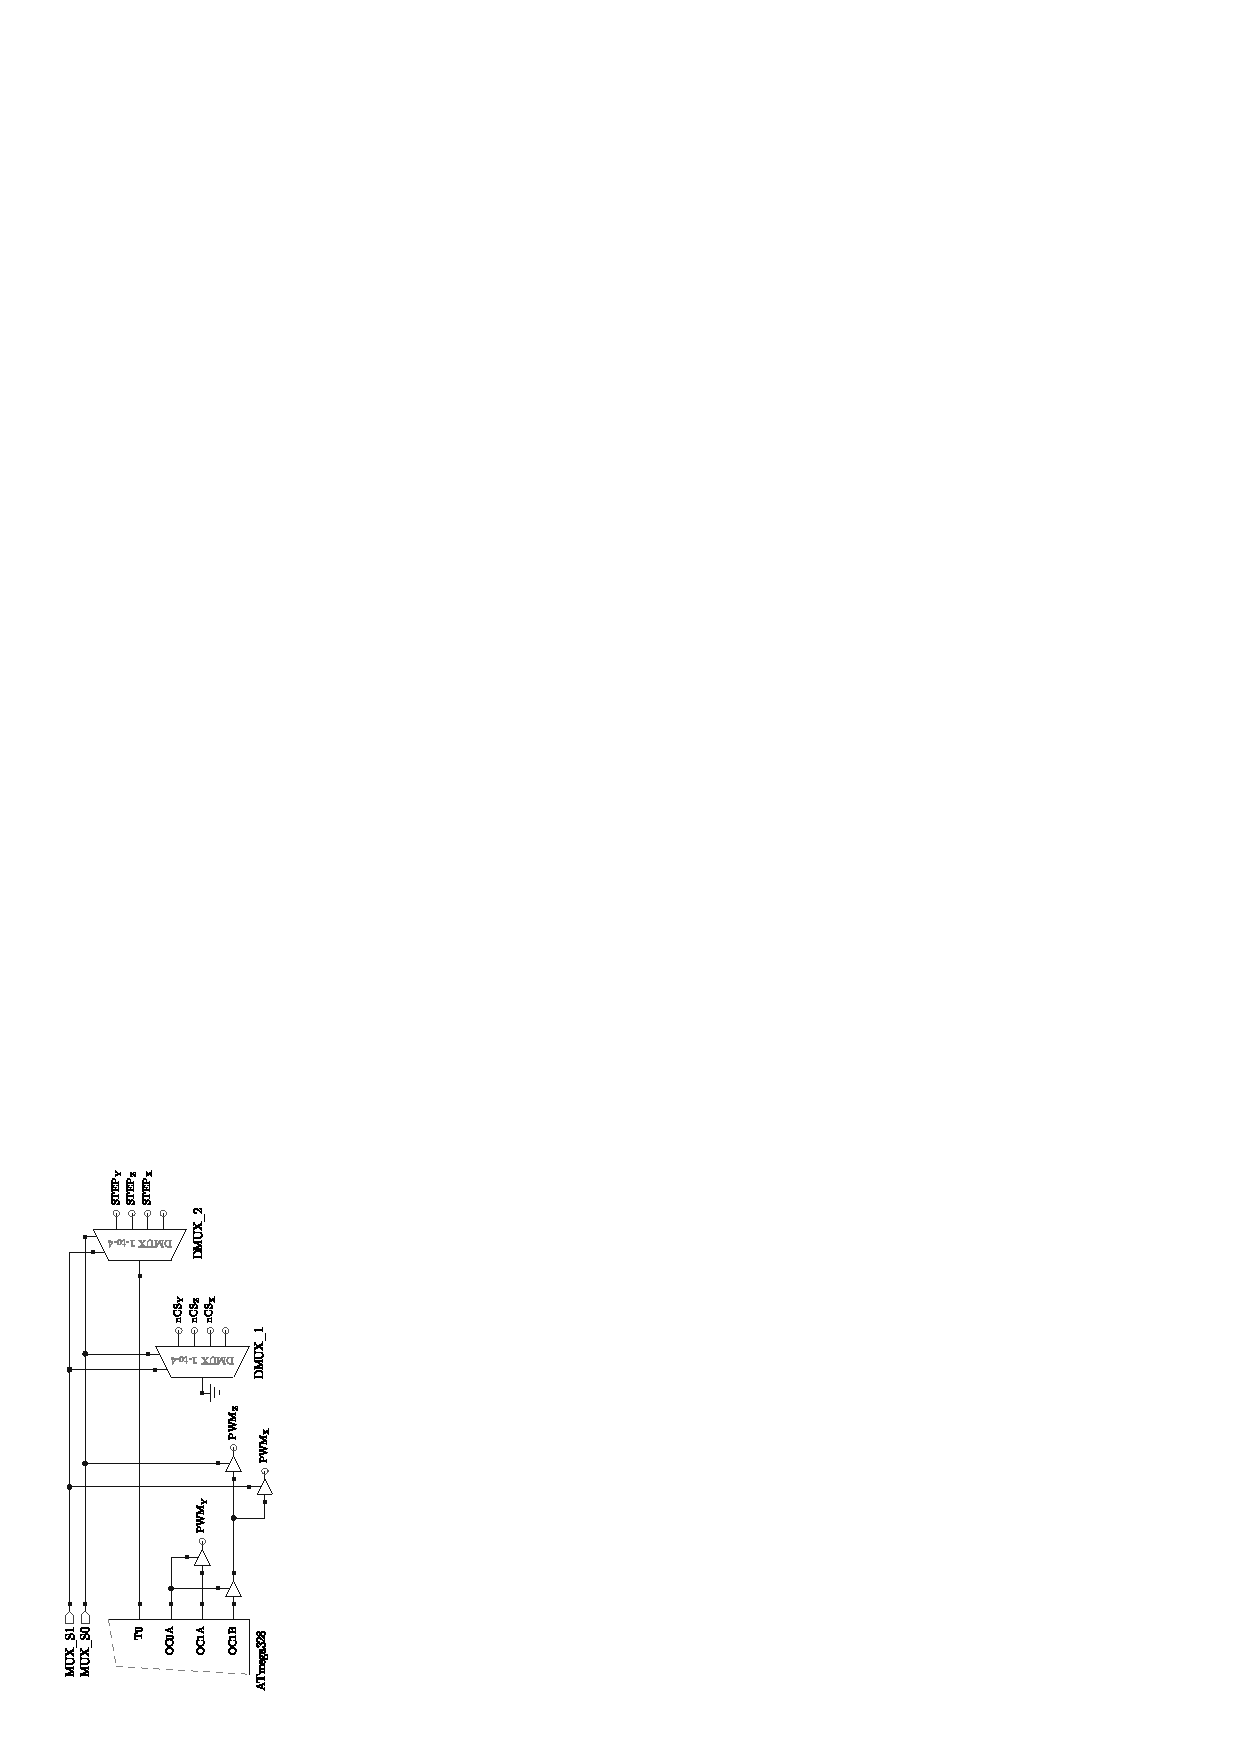
\includegraphics{drive_schem_step-and-pwm}
    \end{center}
\end{figure}

Τα εναπομείναντα κανάλια των δύο αποπολουπλεκτών μπορούν να χρησιμοποιηθούν για
την κάλυψη άλλων αναγκών, δεδομένου ότι η χρήση γίνεται όταν το υποσύστημα
κινητήρων βρίσκεται σε αδράνεια. Για παράδειγμα, το τέταρτο κανάλι του MUX\_1
μπορεί να συνδεθεί με το \nbar{CS} κάποιου άλλου ολοκληρωμένου, ενώ του MUX\_2,
για την ανταλλαγή δεδομένων όταν ο μετρητής βημάτων είναι απενεργοποιημένος.


\section{Εγκλωβισμός και επανάκαμψη}
\label{sec:motor:backtrack}

Η ύπαρξη των κωδικοποιητών κίνησης αιτιολογείται από την ανάγκη ανατροφοδότησης
σχετικά με την πορεία εξέλιξης της μετατόπισης σε κάθε άξονα. Ωστόσο, οι
κωδικοποιητές, αυτοσχέδιοι ή μη, είναι, έως ένα βαθμό, επιρρεπείς σε εσφαλμένες
μετρήσεις, κάτι που καθορίζεται από τη διακριτική τους ικανότητα
\parencite[15--16]{albert11}. Επιπλέον, η υπόθεση ότι, κατά τη μέγιστη κοινή
μετατόπιση, ο αριθμός βημάτων που πραγματοποιείται σε κάθε άξονα είναι ο ίδιος
και για τους δύο, εισάγει επιπρόσθετη πιθανότητα αστοχίας. Ανεξαρτήτως της
συχνότητας εμφάνισης, κρίνεται απαραίτητη η ύπαρξη ενός μηχανισμού ως έσχατη
προστασία κατά της εξώθησης της κεφαλής πέραν των φυσικών ορίων (του πλαισίου)
της συσκευής που οφείλεται σε αδυναμία αναγνώρισης ή παρακολούθησης της
πραγματικής θέσης της κεφαλής.

% nref: Χρήση διακοπτών στην Κατασκευή
Η λύση περιλαμβάνει τη στερέωση μηχανικών διακοπτών σε κάθε πλευρά των κινητών
μερών της συσκευής ώστε κατά την πρόσκρουσή τους με τα άκρα του πλαισίου, αφενός
να απενεργοποιούνται οι κινητήρες και, αφετέρου, να ειδοποιείται ο μικροελεγκτής
για το συμβάν. Και σε αυτήν την περίπτωση, θεωρείται ζωτικής σημασίας η
απενεργοποίηση να συμβαίνει σε επίπεδο υλικού, ενώ το λογισμικό να επεμβαίνει
στην πορεία, όταν ευκαιρήσει. Το σχήμα \ref{fig:motor:limit_switch} παρουσιάζει
τη βασική ιδέα.

\begin{figure}
    \caption{Συνδεσμολογία εγκλωβισμού και επανάκαμψης κινητήρα σε ένα άκρο.
    \label{fig:motor:limit_switch}}
    \begin{center}
    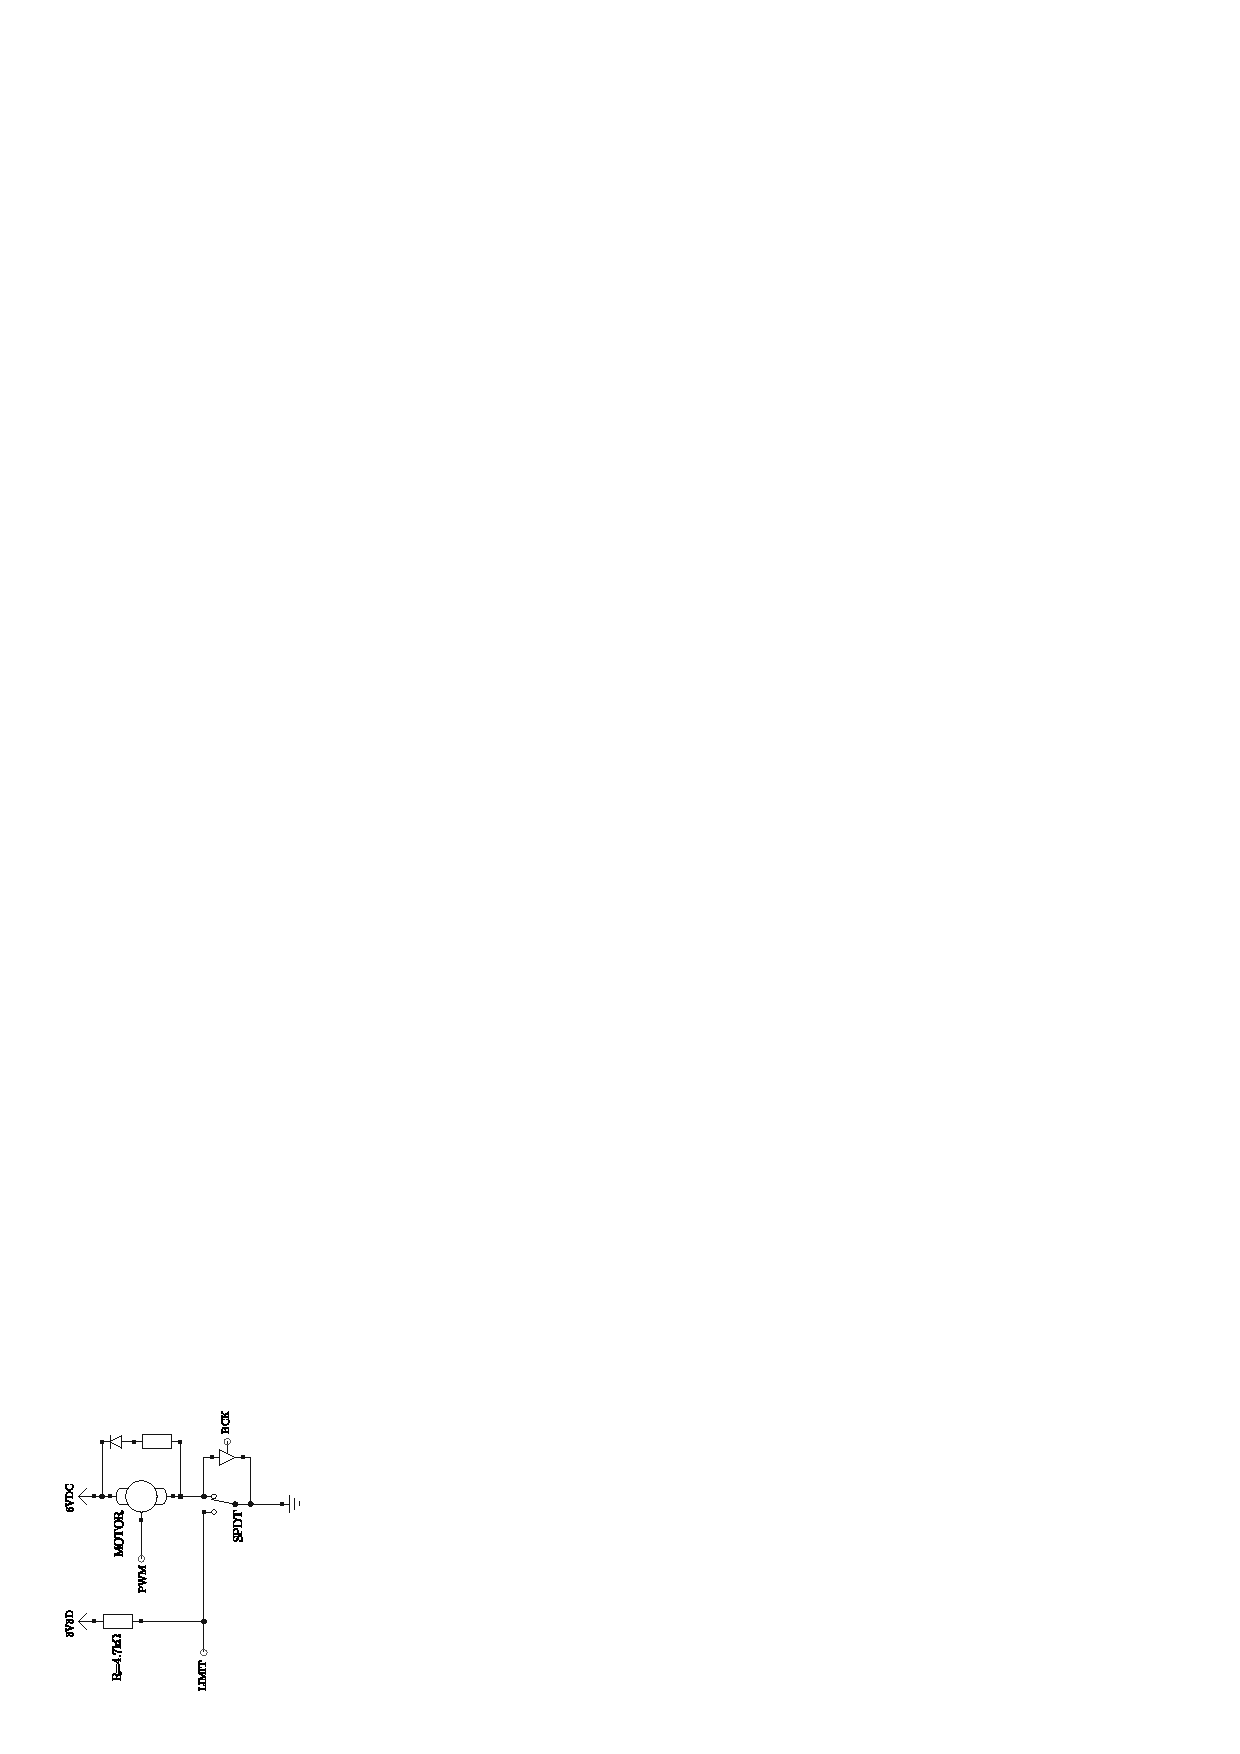
\includegraphics{drive_schem_limit-and-bck}
    \end{center}
\end{figure}

Ο επιλεγμένος διακόπτης είναι SPDT (\textenglish{Single Pole, Double Throw})
και, συνεπώς, διαθέτει τρεις ακροδέκτες· όταν ο διακόπτης είναι ελεύθερος, ο
ακροδέκτης NC (\textenglish{Normally Closed}) συνδέεται με τον COM
(\textenglish{Common}), ενώ όσο βρίσκεται πιεσμένος, ο ακροδέκτης NO
(\textenglish{Normally Open}) συνδέεται με τον COM, ενώ ο NC είναι
αποσυνδεδεμένος. Η τοποθέτηση του διακόπτη στη γραμμή τροφοδοσίας του κινητήρα
επιτρέπει τη μηχανική αποσύνδεσή του όποτε ο διακόπτης πιέζεται.

Προκειμένου να ειδοποιείται ο μικροελεγκτής ότι ο κινητήρας έχει ακινητοποιηθεί,
θα πρέπει η αλλαγή της κατάστασης του διακόπτη να προκαλεί εναλλαγή σε κάποιο
εισερχόμενό του σήμα. Δεδομένου ότι η σύνδεση του ακροδέκτη NO με τον COM θέτει
το σήμα αυτό σε λογικό 0, το σήμα θα πρέπει, υπό φυσιολογικές συνθήκες, να
βρίσκεται σε λογικό 1. Από αυτό αιτιολογείται η ύπαρξη αντιστάτη pull-up στο
σχήμα \ref{fig:motor:limit_switch}, ώστε η γραμμή LIMIT να τίθεται σε λογικό 1,
από προεπιλογή. Από πλευράς ρυθμίσεων, ο μικροελεγκτής αρκεί να διευθετηθεί ώστε
να προκαλείται διακοπή στην εναλλαγή του σήματος του συνδεδεμένου ακροδέκτη
(\textenglish{low triggered} ή \textenglish{edge triggered}).

Η αναγνώριση του συμβάντος από το μικροελεγκτή είναι απαραίτητη ώστε ο κινητήρας
να τίθεται σε κατάλληλη θέση για τη συνέχιση της λειτουργίας του. Αφενός
απαιτείται η αλλαγή του κύκλου εργασίας του σήματος PWM ώστε ο κινητήρας να
περιστρέφεται με φορά αντίθετη αυτής που προκάλεσε τη διακοπή. Ωστόσο, η αλλαγή
του κύκλου εργασίας από μόνη της είναι αδύνατο να επαναφέρει τον κινητήρα καθώς
αυτός είναι μηχανικά αποσυνδεδεμένος από την τροφοδοσία (εξαιτίας του διακόπτη).
Για το λόγο αυτό, παρέχεται ένας ηλεκτρονικός διακόπτης ως εφεδρική σύνδεση με
την τάση αναφοράς (GND). Όταν ο κινητήρας έχει οπισθοδρομήσει αρκετά ώστε να
απεγκλωβιστεί από τον μηχανικό διακόπτη, ο ηλεκτρονικός διακόπτης
απενεργοποιείται και ο κινητήρας είναι σε θέση να λειτουργηθεί κανονικά.

Στο σχήμα απεικονίζεται, επίσης, μία δίοδος επιστροφής συνδεδεμένη στα άκρα του
κινητήρα. Ο λόγος ύπαρξής της είναι η εξομάλυνση παλμών που δημιουργούνται κατά
την κατάρρευση του μαγνητικού πεδίου του πηνίου του κινητήρα όταν αυτός
αποσυνδέεται από την τροφοδοσία \parencite[130--132]{kuphaldt09semi}. Ωστόσο,
κρίνεται ότι στην περίπτωση της υλοποίησης, η οποία χρησιμοποιεί σερβοκινητήρες,
η ανάγκη για συμπερίληψή τους είναι μικρή και, τελικά, αποκλείονται από αυτήν.

\subsection{Προσαρμογή στις ανάγκες της υλοποίησης}

Η προαναφερθείσα συνδεσμολογία αγνοεί το γεγονός ότι απαιτούνται δύο
ανασταλτικοί διακόπτες SPDT ανά κινητήρα -- έναν για κάθε άκρο -- καθώς και το
γεγονός ότι ο κινητήρας Z κινείται μόνο εφόσον οι άλλοι δύο βρίσκονται σε
ηρεμία. Το τελευταίο θα μπορούσε να χρησιμοποιηθεί για τη μείωση του αριθμού των
παραγόμενων σημάτων. Στο σχήμα \ref{fig:motor:limit_switch_final} παρουσιάζεται
η τελική συνδεσμολογία. Παρατηρείται ότι οι ανασταλτικοί διακόπτες των αξόνων X
και Z συνδέονται σε σειρά και ότι χρησιμοποιείται μόνο ένας ηλεκτρονικός
διακόπτης για την εφεδρική σύνδεση με την τάση αναφοράς (BCK\tsub{XZ}).
Αντιστοίχως, δεσμεύεται μόνο ένας ακροδέκτης του μικροελεγκτή για την ειδοποίηση
εγκλωβισμού κάποιου εκ των δύο κινητήρων (LIMIT\tsub{XZ}).

\begin{figure}
    \caption{Πλήρης συνδεσμολογία εγκλωβισμού και επανάκαμψης.
    \label{fig:motor:limit_switch_final}}
    \begin{center}
    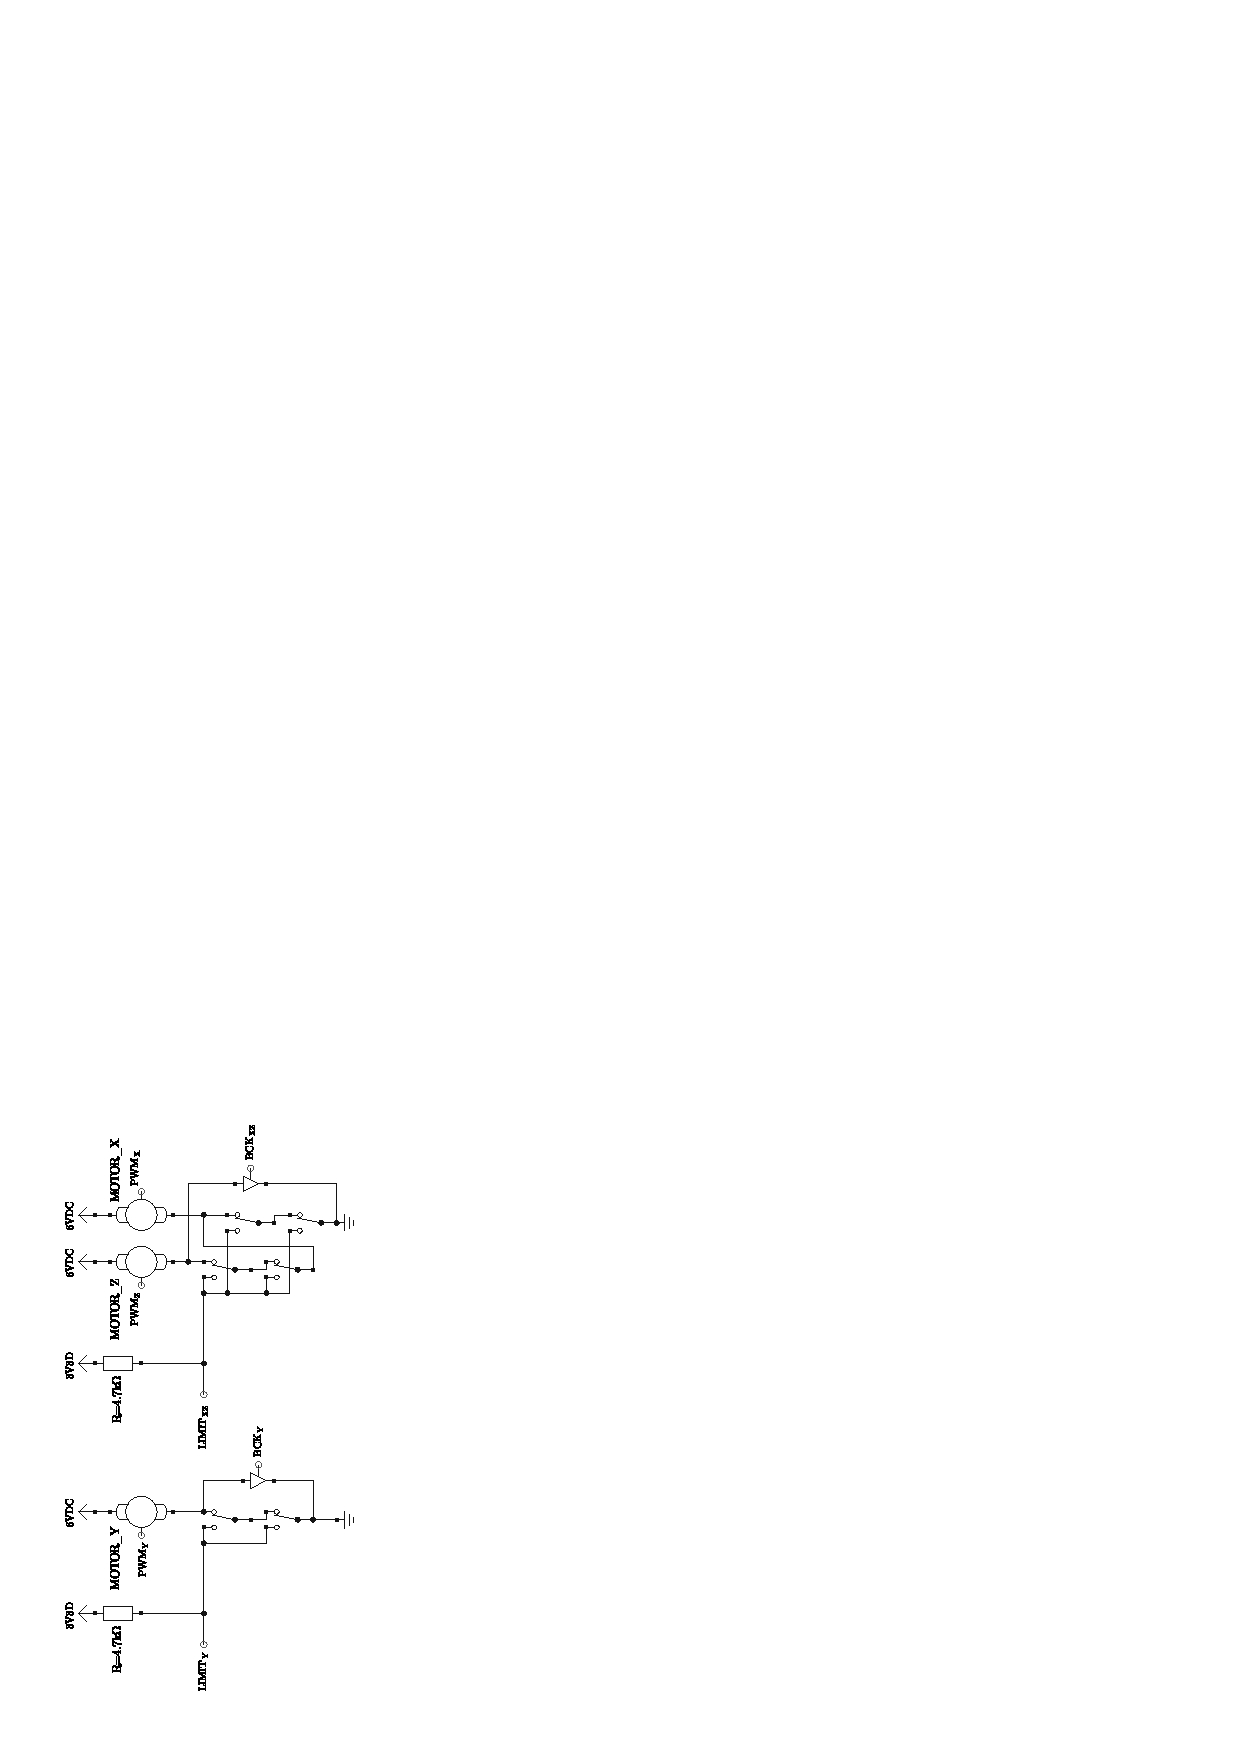
\includegraphics{drive_schem_limit-and-bck_all}
    \end{center}
\end{figure}

Ο λόγος για τη συγχώνευση των κυκλωμάτων των κινητήρων X και Z αντί των Y και Z
είναι η διευκόλυνση της φυσικής διασύνδεσης των διακοπτών λόγω της εγγύτητας των
δύο αξόνων.
% nref: Διάταξη αξόνων (Z over X).
Η σύνδεση X και Y, σαφώς, απορρίπτεται, καθώς αυτοί οι δύο κινητήρες δύνανται να
τεθούν σε λειτουργία ταυτόχρονα και θα ήταν, συνεπώς, αδύνατο να εντοπιστεί
ποιος από τους δύο έχει εγκλωβιστεί.

Το βασικό μειονέκτημα της επιλεγμένης μεθόδου είναι ότι επιτρέπει την αναγνώριση
του κυκλώματος κινητήρων και όχι του συγκεκριμένου διακόπτη που προκαλεί τον
εγκλωβισμό. Συνεπώς, εφόσον οι κινητήρες τίθενται σε κίνηση από το μικροελεγκτή
και στην πορεία προκύπτει εγκλωβισμός, η κατάσταση είναι δυνατό να αναστραφεί.
Ωστόσο, αν κατά την εκκίνηση της συσκευής κάποιος κινητήρας είναι εγκλωβισμένος,
αυτός ο μηχανισμός από μόνος του είναι ανεπαρκής για την επανάκαμψή του. Η
παρούσα υλοποίηση αρκείται σε αυτόν το μηχανισμό χωρίς να καταβάλει προσπάθεια
επανάκαμψης στην προαναφερθείσα περίπτωση.

\subsection{Αναγγελία εγκλωβισμού}
\label{subsec:motor:limit-pin-change}

Αναφέρθηκε προηγουμένως η ανάγκη διευθέτησης του μικροελεγκτή για την απόκριση
του στην εναλλαγή των σημάτων LIMIT\tsub{XZ} και LIMIT\tsub{Y}. Σύμφωνα με το
εγχειρίδιο του μικροελεγκτή της \textcite[71]{atmel13}, εξωτερικές διακοπές
είναι δυνατό να ενεργοποιηθούν για εισερχόμενες παρυφές (\textenglish{edge
triggered}) σε οποιοδήποτε ακροδέκτη PCINT ή, επιπροσθέτως, για οποιαδήποτε
λογική αλλαγή στους ακροδέκτες INT0 και INT1. Προτιμάται η χρήση δύο PCINT
ακροδεκτών καθώς καλύπτουν τις απαιτήσεις ενώ, ταυτόχρονα, επιτρέπουν τη χρήση
των ειδικών ακροδεκτών INT0 και INT1 σε περιπτώσεις όπου διακοπή σε εναλλαγή
σήματος είναι ακατάλληλη.

Το σύνολο των ακροδεκτών PCINT διαμοιράζεται σε τρεις ομάδες. Η εναλλαγή του
σήματος ενός οποιουδήποτε ακροδέκτη κάθε ομάδας προκαλεί την εκτέλεση της ίδιας
ρουτίνας εξυπηρέτησης, εφόσον το bit της αντίστοιχης ομάδας του καταχωρητή PCICR
(\textenglish{Pin Change Interrupt Conrol Register}) έχει τεθεί. Επιπλέον, με
τους καταχωρητές PCMSK (\textenglish{Pin Change Mask Register}) -- 1, 2 και 3 --
προσδιορίζονται ποιοι PCINT ακροδέκτες κάθε ομάδας είναι επιθυμητό να προκαλούν
διακοπή.

Το γεγονός ότι όλοι οι ακροδέκτες του μικροελεγκτή αντιστοιχίζονται με κάποιον
PCINT, καθιστούν εύκολη την επιλογή και ανάθεση δύο εξ αυτών στα σήματα
LIMIT\tsub{XZ} και LIMIT\tsub{Υ}. Ωστόσο, προτιμώνται δύο ακροδέκτες PCINT που
ανήκουν στην ίδια ομάδα με αποτέλεσμα να καλείται η ίδια ρουτίνα εξυπηρέτησης
ώστε η αναγνώριση του εγκλωβισμένου κινητήρα να επαφίεται στο ίδιο το λογισμικό
(σαφώς με τη βοήθεια των σημάτων).
